%%%%%%%%%%%%%%%%%%%%%%%%%%%%%%%%%%%%%%%%%%%%%%%%%%%%%%%%%%%%%%%%%%%%%%%%%%%%%%%%%%%%%%%%%%%%%%%%%%%%%%%
% Manuel d'Utilisation
% Bitume Legends Project
% CarrEniX
% Juin 2022
%%%%%%%%%%%%%%%%%%%%%%%%%%%%%%%%%%%%%%%%%%%%%%%%%%%%%%%%%%%%%%%%%%%%%%%%%%%%%%%%%%%%%%%%%%%%%%%%%%%%%%%

\documentclass[a4paper,12pt]{article}

\usepackage[utf8]{inputenc}
\usepackage[french]{babel}
\usepackage{geometry}
\usepackage{lipsum}
\usepackage{mathtools}
\usepackage[T1]{fontenc}
\usepackage{url}
\usepackage{longtable}
\usepackage[aboveskip=.5cm]{caption}
\usepackage{pdflscape}
\usepackage{xcolor}
\usepackage{fancyhdr}
\usepackage{graphicx,color}
\graphicspath{{../Medias}}

\newcommand{\hsp}{\hspace{20pt}}
\newcommand\esc{\button{ECHAP}}
\newcommand{\HRule}{\rule{\linewidth}{0.5mm}}
\newcommand{\btmlgs}{\textsl{Bitume Legends}}
\newcommand{\AI}{Intelligence Artificielle}
\newcommand{\FL}{\textsl{FL Studio 20}}
\newcommand{\CEX}{\textsc{CarrEniX}}
\newcommand{\SITE}{\(\mathtt{btms.games}\)}
\newcommand{\report}{Manuel d'Utilisation}
\renewcommand{\listfigurename}{Table des Annexes}
\renewcommand{\contentsname}{Table des Matières}
\newcommand\ytl[2]{\parbox[b]{10em}{\hfill{\color{cyan}\bfseries\sffamily 
    #1}~$\cdots\cdots$~}\makebox[0pt][c]{$\bullet$}\vrule\quad 
    \parbox[c]{5cm}{\vspace{7pt}\color{red!40!black!80}\raggedright\sffamily #2\\[7pt]}\\[-3pt]}
\newcommand\button[1]{\fbox{\texttt{#1}}}
\newcommand\room{\textsl{room}}


\pagestyle{fancy}
\lhead{\report}
\rhead{{\CEX}\\{\btmlgs}}   

\begin{document}  

    % Homepage
    \begin{titlepage}
        \begin{center}
            
\includegraphics[scale=0.7]{logo192.png}\\[0.5cm]
            \textsc{\Large \report}\\[1.5cm]

            \HRule \\[0.4cm]
            { \LARGE \bfseries \btmlgs \\[0.4cm] }

            \HRule \\[2cm]
        
            \textsc{by \Large \CEX}\\[7cm]
            \HRule\\
            Lien pour télécharger le jeu: \url{https://btms.games/telechargement.html}
        \end{center}
    \end{titlepage}

    \tableofcontents
    \clearpage

    \addcontentsline{toc}{section}{Introduction}
    \section*{Introduction}
        Ce document est un manuel d'utilisation de \btmlgs.
        Pour installer \btmlgs, merci de se référer au manuel d'installation.

    \section{Commandes de base}
        Pour utiliser \btmlgs, il y a certaines commandes à connaître.
        Celles ci dépendent de la disposition du clavier.

        \subsection{Contrôle de la voiture}
            \begin{center}
                \begin{tabular}[c]{|| c | c | c ||}
                    \hline\hline
                    Commande & AZERTY & QWERTY\\\hline\hline
                    Avancer & Z & W\\\hline
                    Reculer & S & S\\\hline
                    Tourner à droite & Q & A\\\hline
                    Tourner à gauche & D & D\\\hline
                    Klaxon & H & H\\\hline\hline
                \end{tabular}
            \end{center}

        \subsection{Touche \esc}
            \begin{itemize}
                \item Dans une course, la touche \esc\; peut être utilisée
                    pour mettre le jeu en pause et ouvrir le menu pause du jeu.
                    Cela permet de quitter la course, ou bien de la recommencer.
            
                \item Dans les menus, la touche \esc\; permet de quitter le menu ouvert,
                    et de retourner au menu principal.
            \end{itemize}

        \subsection{Autres touches utiles}
            \begin{itemize}
                \item La touche \button{ENTRÉE} permet de valider un choix de voiture
                    dans le garage, ou encore valider un nom de \textit{room} dans le menu
                    du \textsl{Multiplayer}.

                \item Les touches \fbox{$\triangleleft$} et \fbox{$\triangleright$} permettent
                    de choisir une voiture dans le garage sans passer par les flèches visibles.
            \end{itemize}

    \clearpage

    \section{Se repérer dans...}
        \subsection{...le menu principal}
            \begin{figure}[!h]
                \centering
                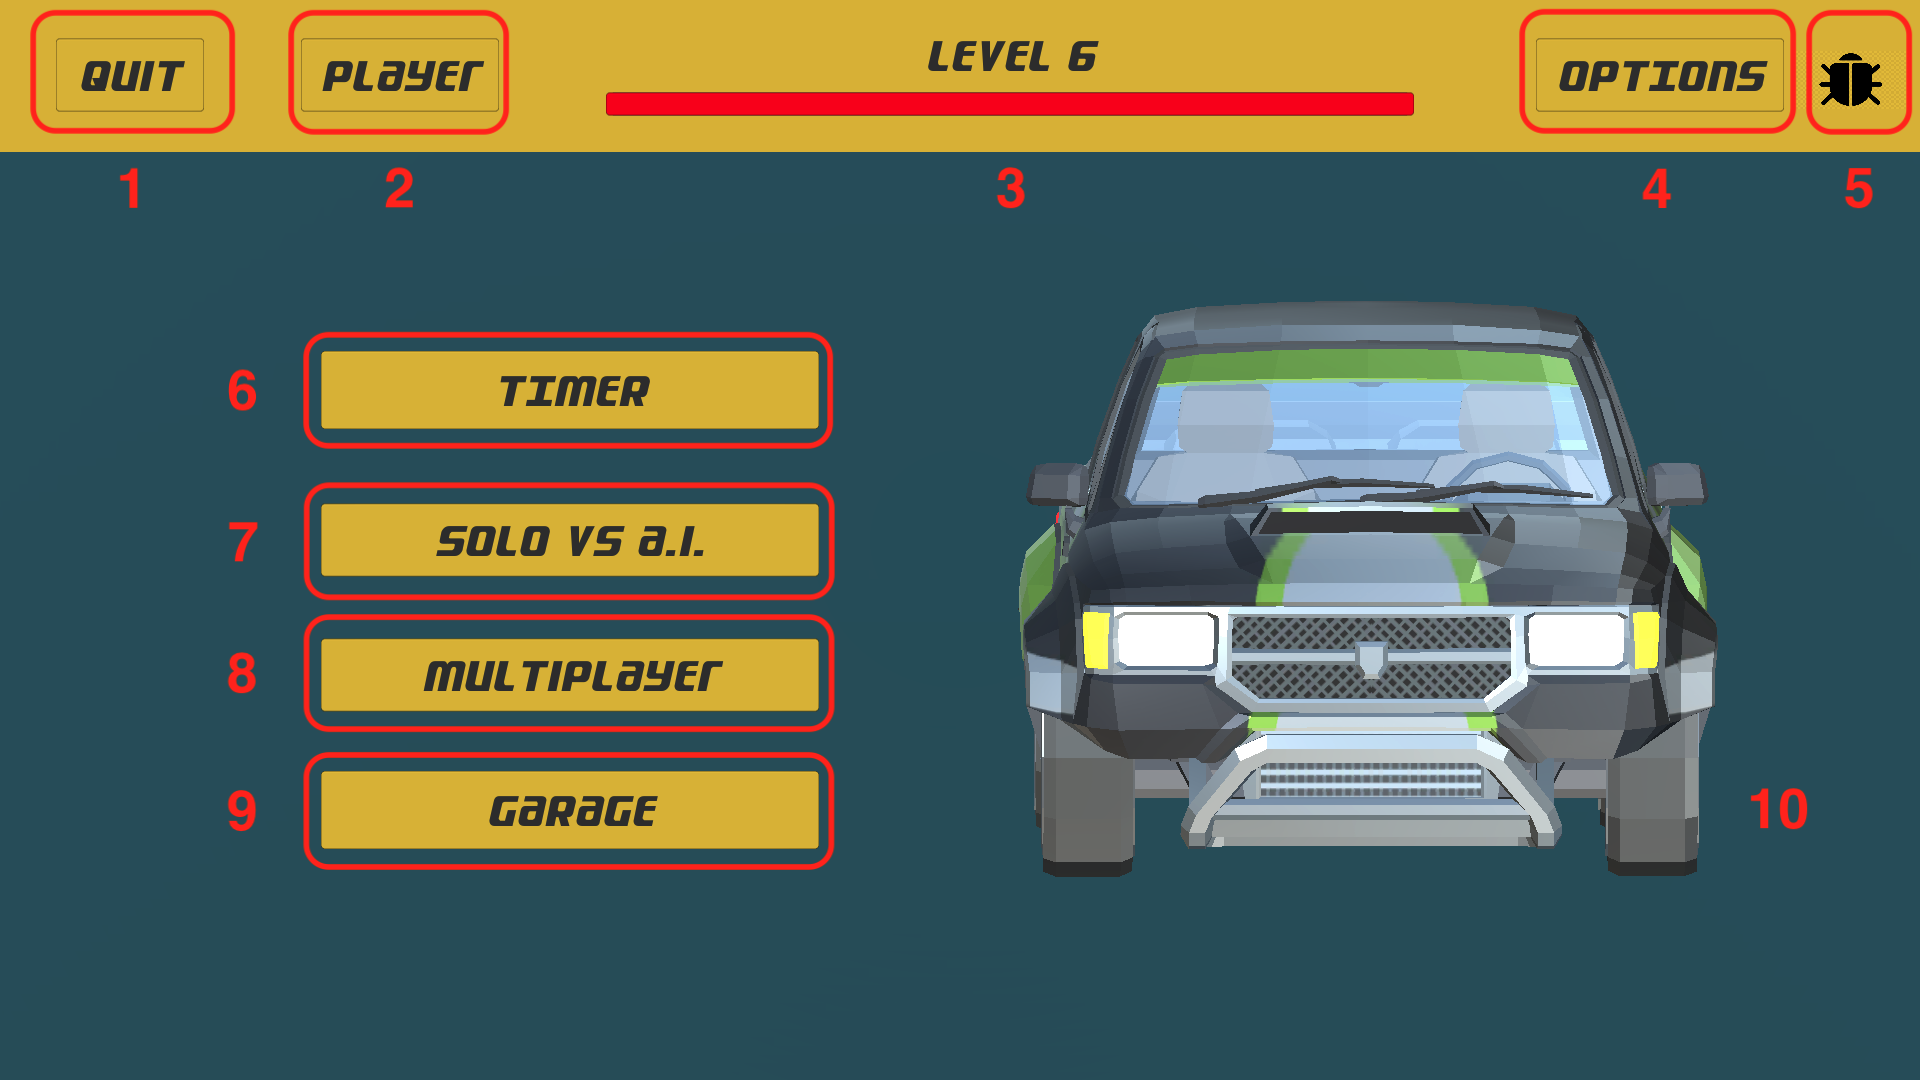
\includegraphics[scale=0.2]{utils_menu_principal.png}
                \caption{Menu principal}
            \end{figure}
            \begin{enumerate}
                \item \button{Quit}: Permet de quitter le jeu.
                \item \button{Player}: Permet voir les statistiques du joueur.
                \item \button{Level}: Permet de voir le niveau et l'expérience du joueur.
                \item \button{Options}: Permet de configurer le jeu.
                \item \button{Bug}: Permet de remonter un bug.
                \item \button{Timer}: Pour jouer contre la montre.
                \item \button{Solo vs A.I.}: pour jouer contre une IA.
                \item \button{Multiplayer}: Pour jouer avec ses amis.
                \item \button{Garage}: Permet de choisir sa voiture avant la course.
                \item \button{The car}: La voiture qui est choisie pour jouer.
            \end{enumerate}

        \clearpage
        \subsection{...le menu \textsl{Timer} / \textsl{Solo vs A.I.}}
            \begin{figure}[h]
                \centering
                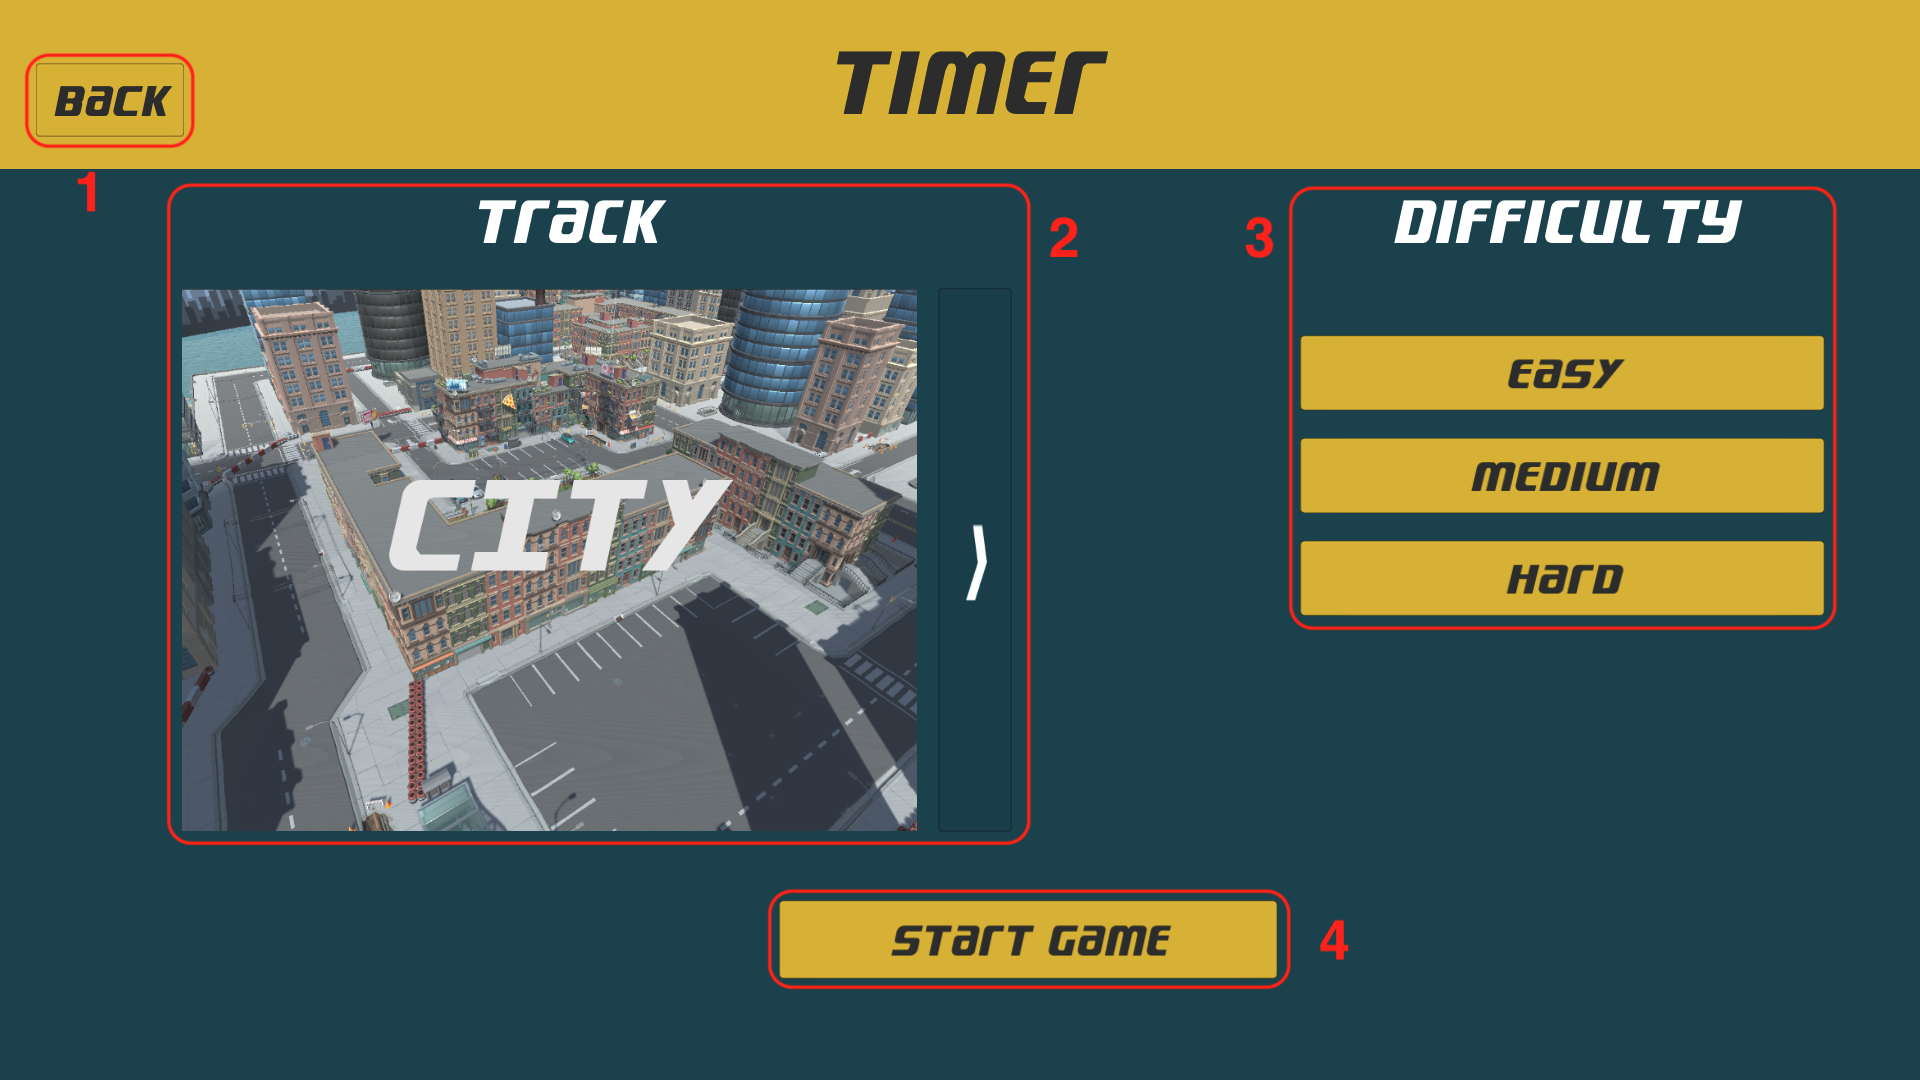
\includegraphics[scale=0.2]{timermode.png}
                \caption{Menu du \textsl{Timer} / \textsl{Solo vs A.I.}}
            \end{figure}
            \begin{enumerate}
                \item \button{Back}: Permet de revenir au menu principal.
                \item \button{Track}: Permet de choisir un circuit pour la course.
                \item \button{Difficulty}: Permet de sélectionner la difficulté de la course.
                \item \button{Start Game}: Lance la course.
            \end{enumerate}

        \clearpage
        \subsection{...le menu \textsl{Multiplayer}}
            \begin{figure}[h]
                \centering
                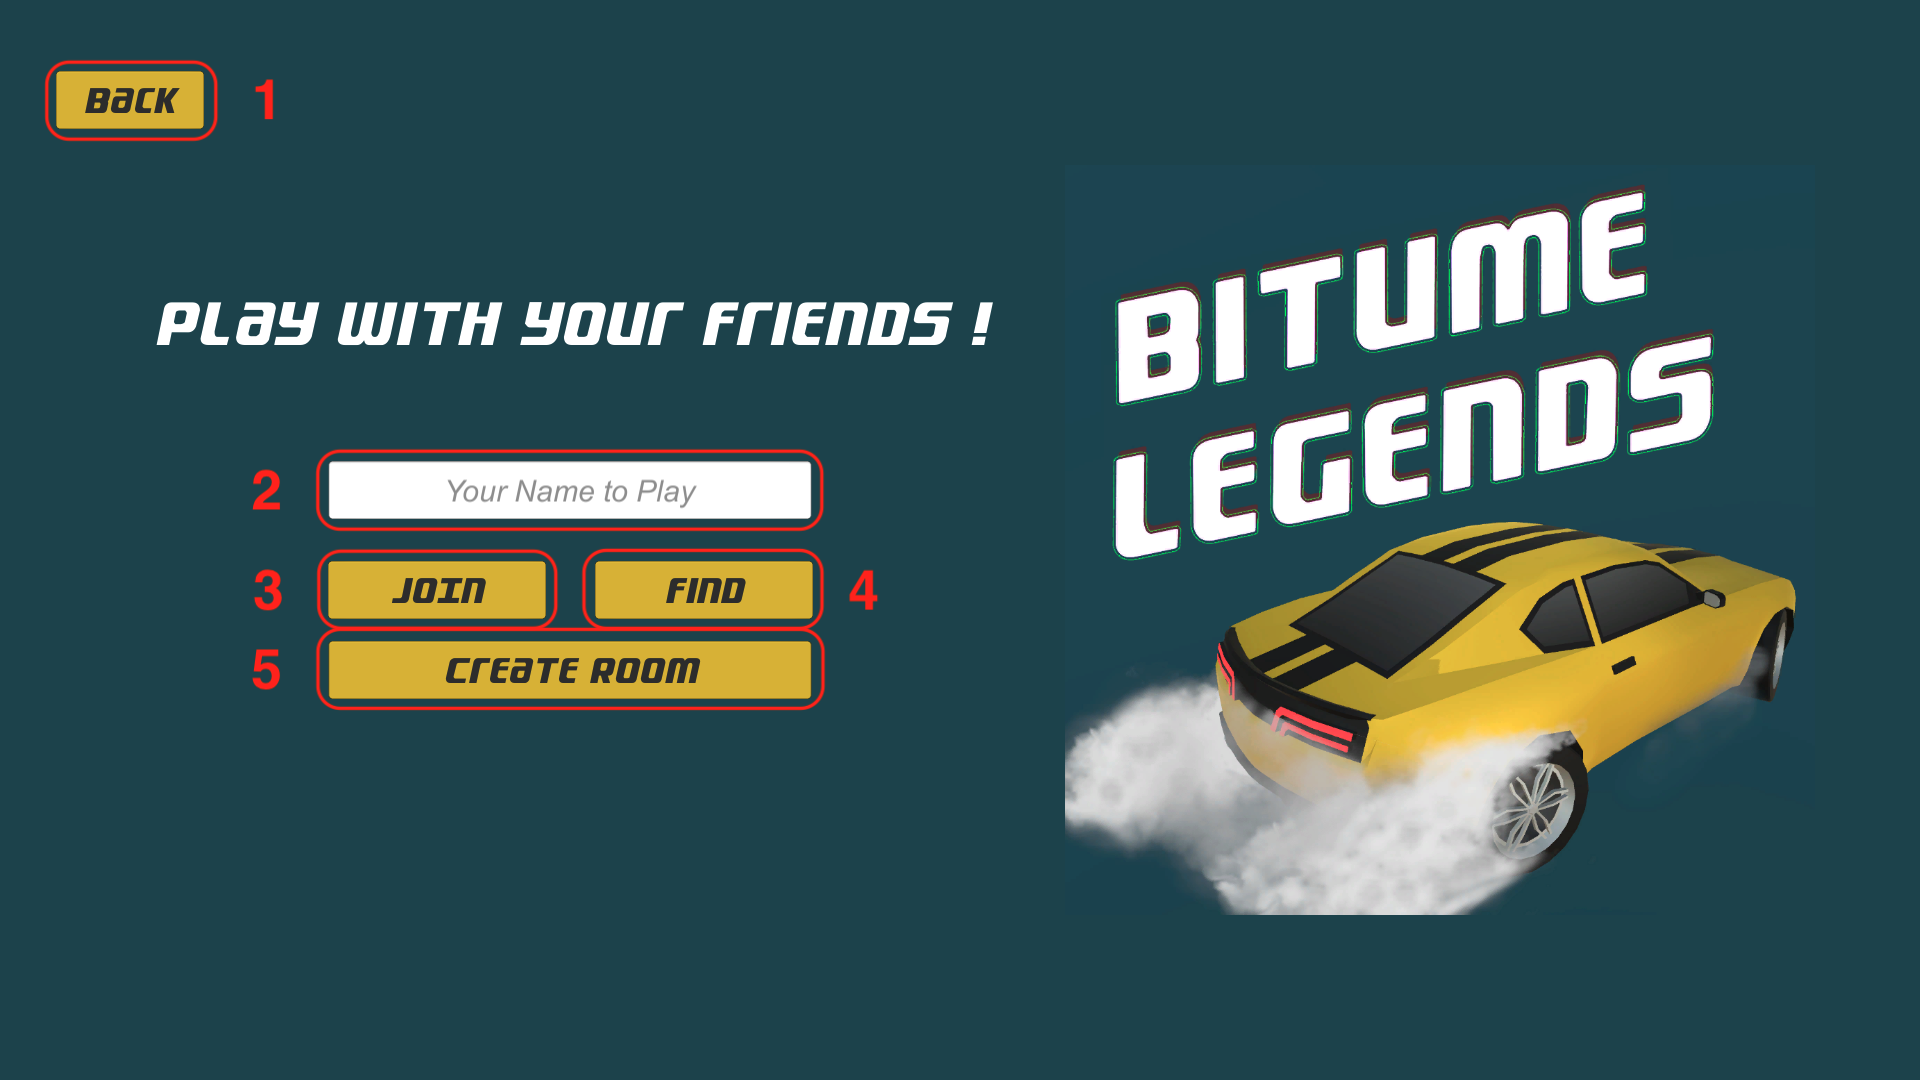
\includegraphics[scale=0.2]{multi_menu.png}
                \caption{Menu \textsl{Multiplayer}}
            \end{figure}
            Dans ce document, le mot \room\;est utilisé pour désigner une instance
            de jeu en multijoueur, c'est à dire une partie de jeu.
            \begin{enumerate}
                \item \button{Back}: Permet de revenir au menu principal.
                \item \button{Name}: Rentrer ici le pseudo du joueur pour la course.
                \item \button{Join}: Permet de se connecter à une \room\; si on connaît le nom de celle-ci.
                \item \button{Find}: Permet de trouver une \room\; ouverte.
                \item \button{Create}: Permet de créer une \room.
            \end{enumerate}
            
        \clearpage
        \subsection{...le \textsl{Garage}} 
            \begin{figure}[h]
                \centering
                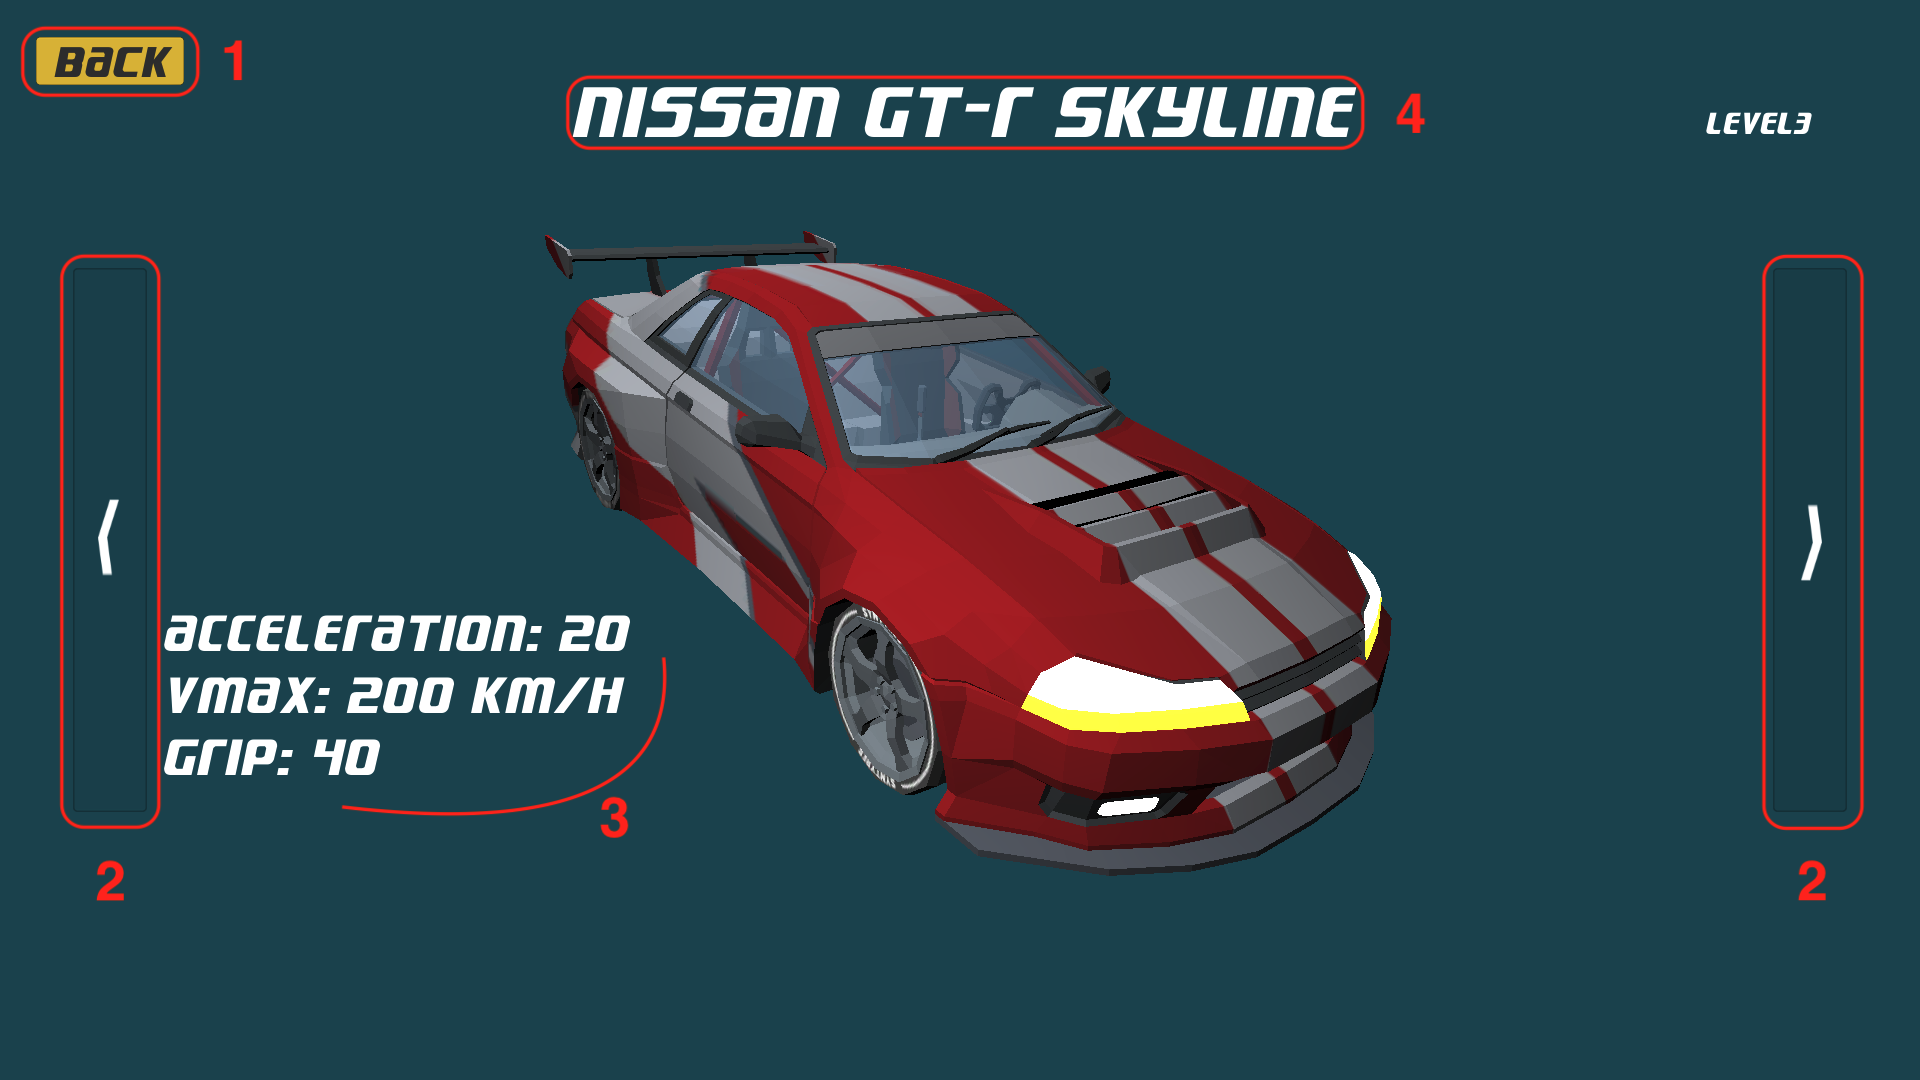
\includegraphics[scale=0.2]{garage.png}
                \caption{Garage}
            \end{figure}
            \begin{enumerate}
                \item \button{Back}: Permet de revenir au menu principal en validant la voiture affichée.
                \item \fbox{$\triangleleft$} / \fbox{$\triangleright$}: Permet de choisir une voiture pour la course.
                \item \button{Specifications}: Indique les spécifications de la voiture.
                \item \button{Name}: Indique le nom de la voiture.
                \item \button{Car}: Montre la voiture en question.
                \item \button{Lock}: indique que le joueur n'a pas assez d'expérience pour débloquer la voiture.
            \end{enumerate}

        \clearpage
        \subsection{...le menu \textsl{Options}}
            \begin{figure}[h]
                \centering
                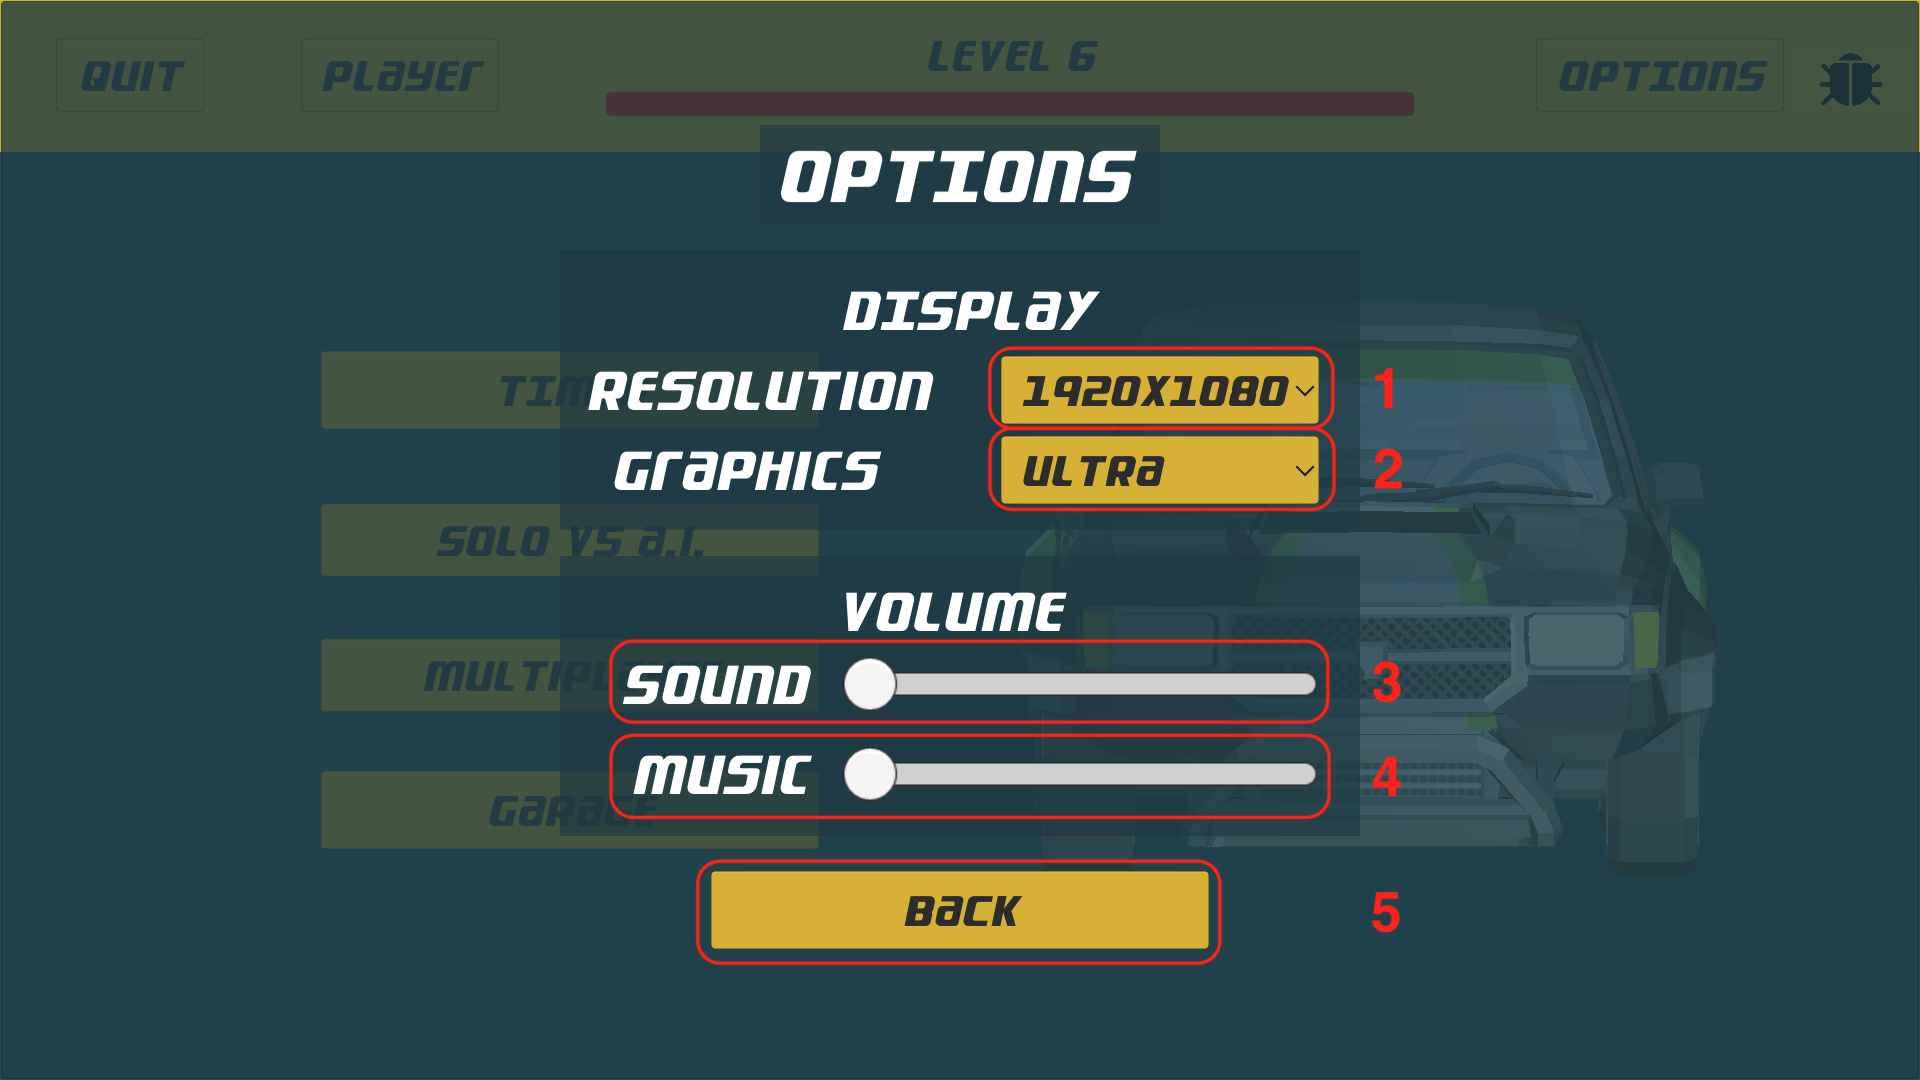
\includegraphics[scale=0.2]{option_menu.png}
                \caption{Menu \textsl{Options}}
            \end{figure}
            \begin{enumerate}
                \item \button{Resolution}: Permet de choisir une résolution parmi celles proposées.
                \item \button{Graphics}: Permet de sélectionner une qualité de graphismes.
                \item \button{Sound}: Permet de régler le volume des sons du jeu.
                \item \button{Music}: Permet de régler le volume de la musique.
                \item \button{Back}: Permet de revenir au menu principal.
            \end{enumerate}

        \clearpage
        \subsection{...le menu \textsl{Player}}
            \begin{figure}[h]
                \centering
                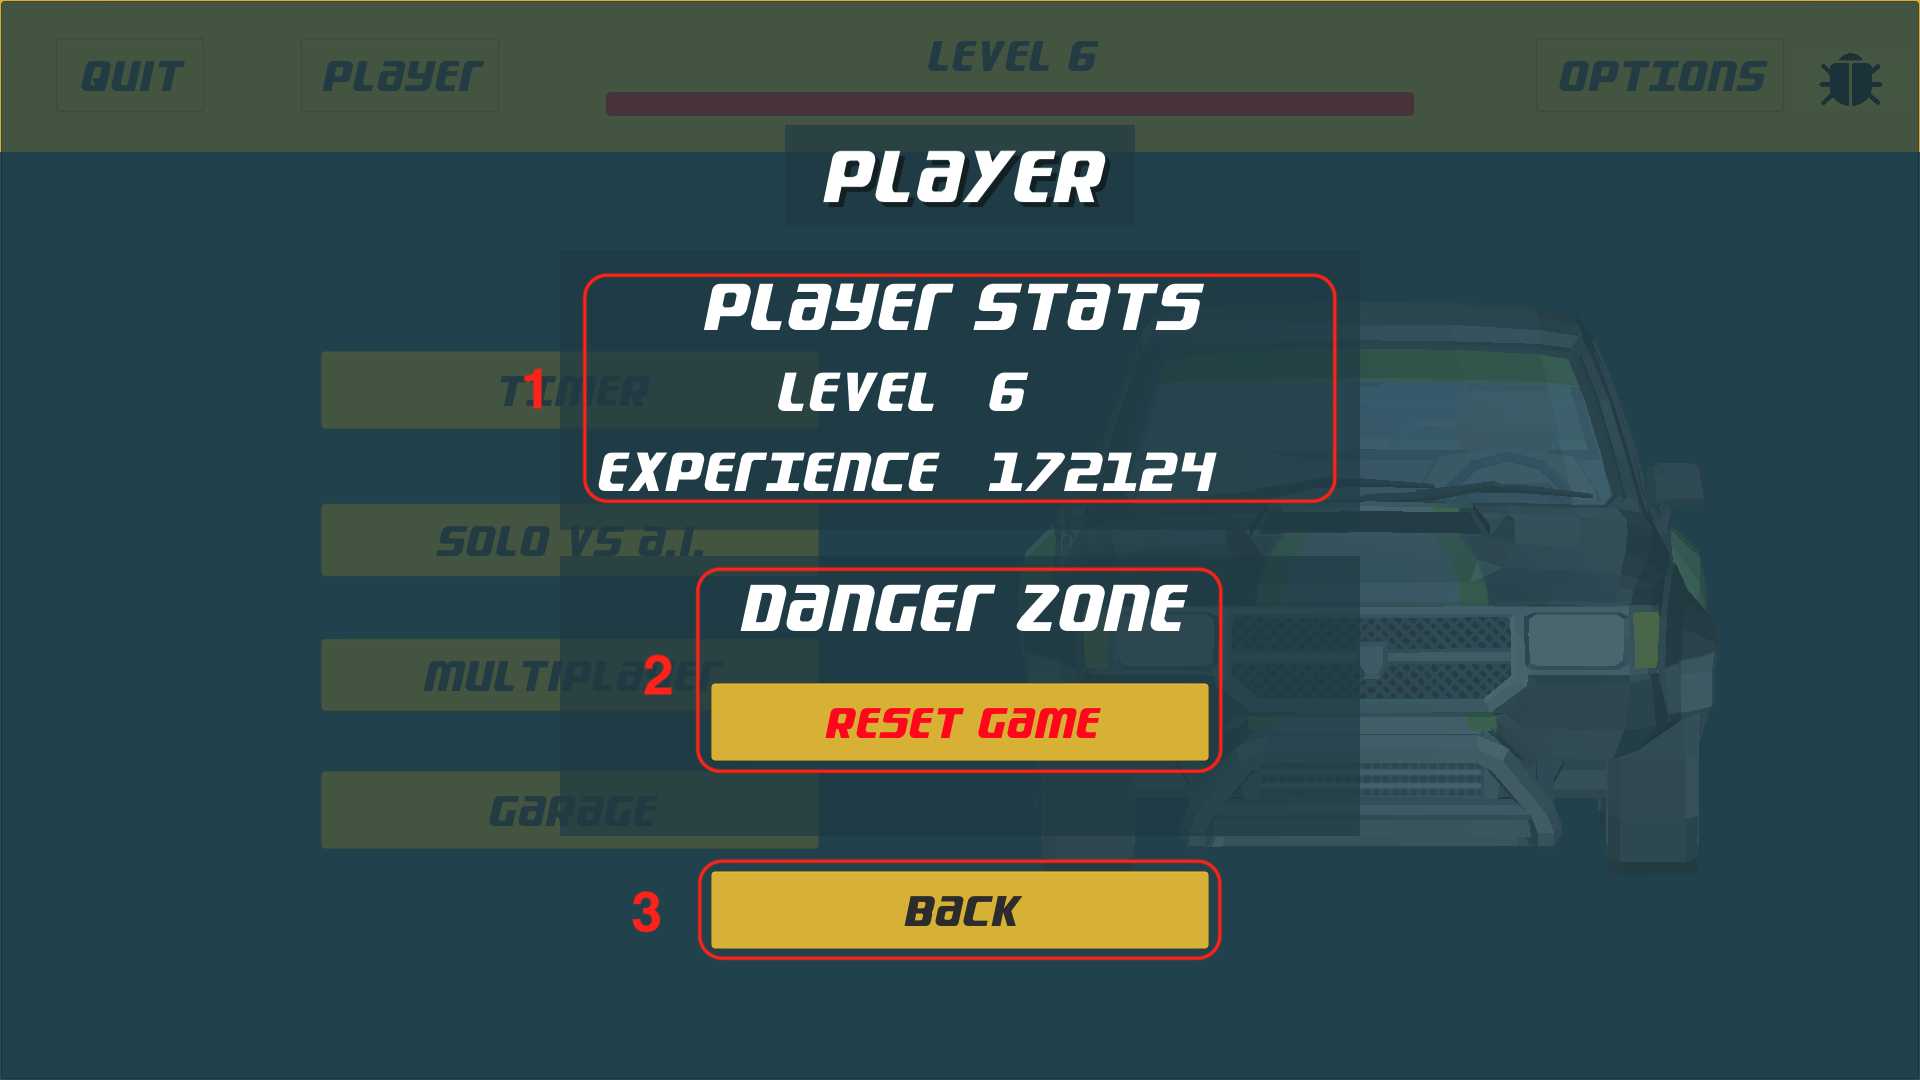
\includegraphics[scale=0.2]{player_menu.png}
                \caption{Menu \textsl{Player}}
            \end{figure}
            \begin{enumerate}
                \item \button{Stats}: Indique l'expérience du joueur ainsi que son niveau.
                \item \button{Reset}: Permet de remettre le jeu à 0 pour recommencer la progression.
                \item \button{Back}: Permet de revenir au menu principal.
            \end{enumerate}

        \clearpage
        \subsection{...le menu \textsl{Pause}}
            \begin{figure}[h]
                \centering
                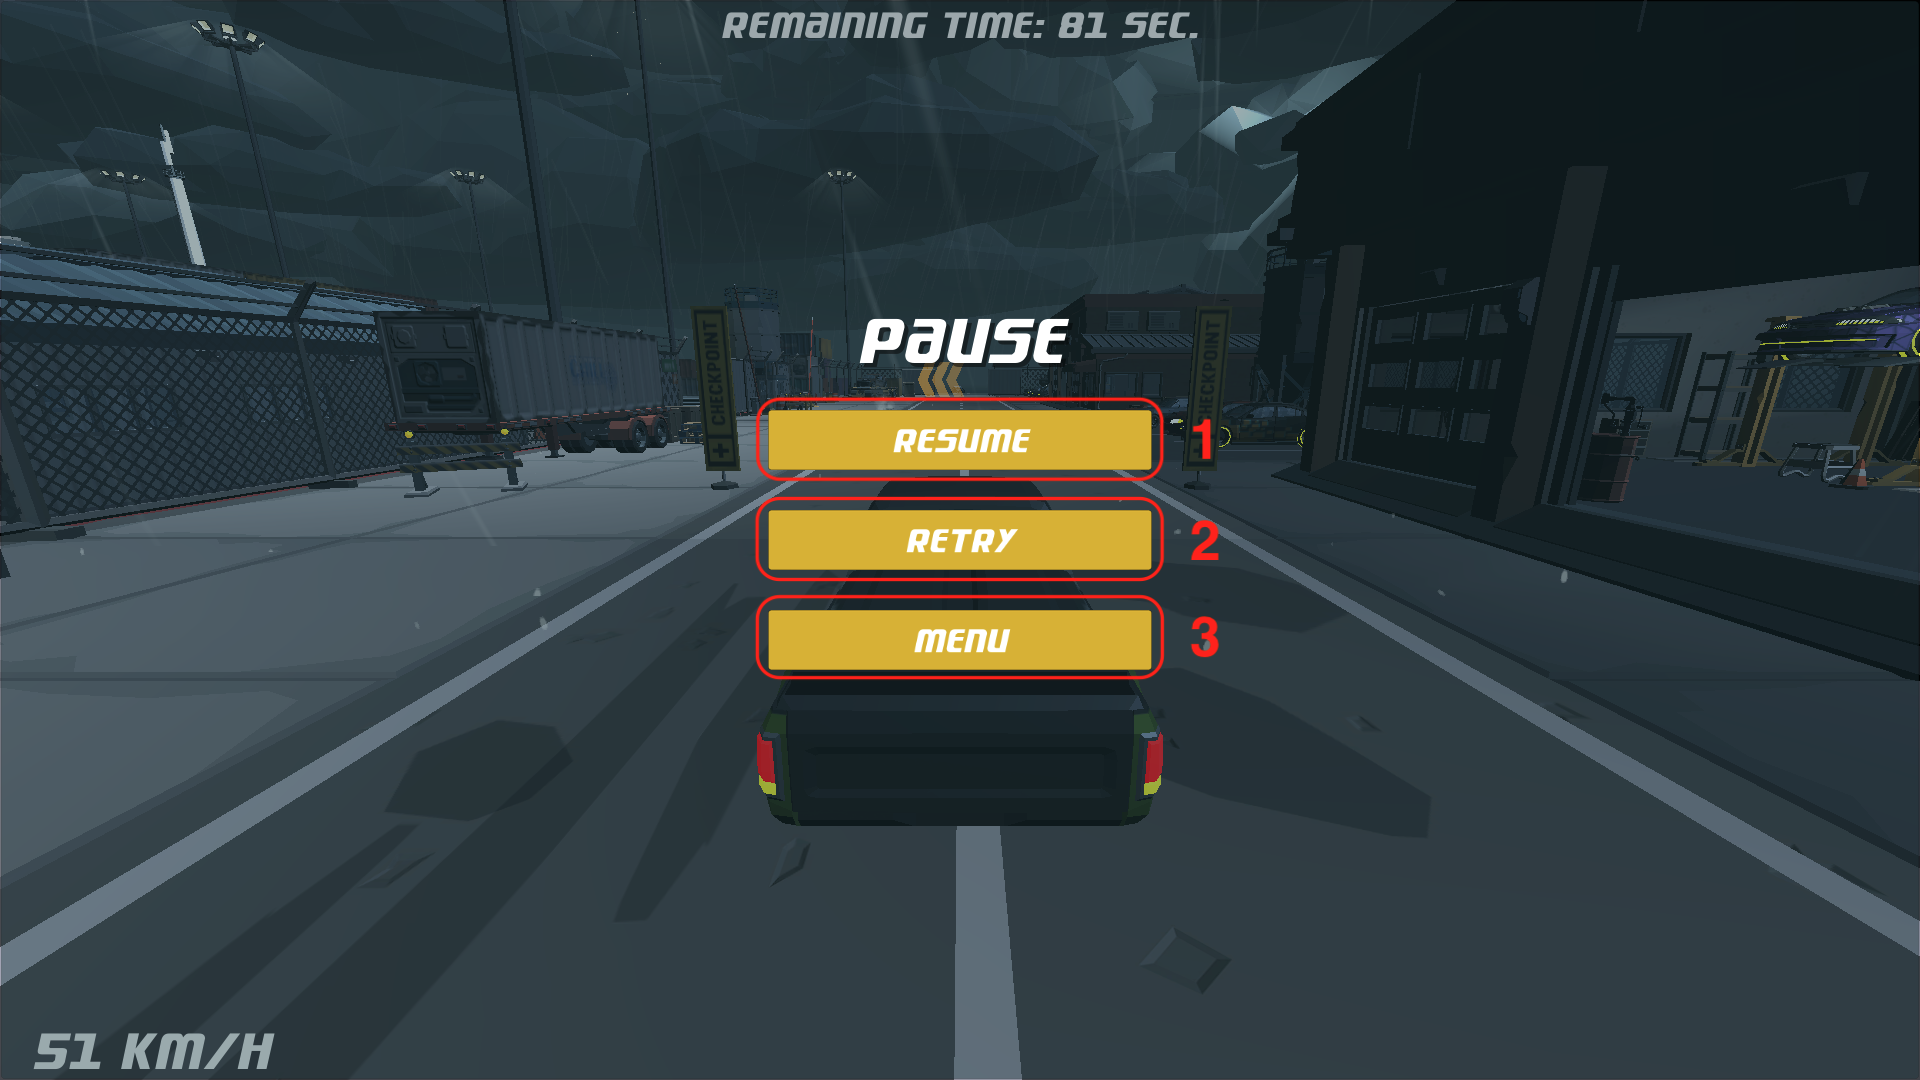
\includegraphics[scale=0.2]{pause_menu.png}
                \caption{Menu \textsl{Pause}}
            \end{figure}
            \begin{enumerate}
                \item \button{Resume}: Permet de reprendre la course.
                \item \button{Retry}: Relance la course depuis le début.
                \item \button{Menu}: Permet de revenir au menu principal.
            \end{enumerate}

    \clearpage
    \section{Lancer une partie en mode \textsl{Timer} ou \textsl{Solo vs A.I.}}
        \begin{enumerate}
            \item \textbf{Ouvrir} le \textsl{Garage}.
            \item \textbf{Choisir} une voiture.
            \item \textbf{Revenir} sur le menu principal.
            \item \textbf{Choisir} un mode de course.
            \item \textbf{Choisir} un circuit.
            \item \textbf{Choisir} une difficulté.
            \item \textbf{Lancer} le jeu.
            \item \textbf{Gagner}!
        \end{enumerate}
    \section{Lancer une partie en mode \textsl{Multiplayer}}
        \subsection{Pour créer une partie}
            \begin{enumerate}
                \item \textbf{Ouvrir} le \textsl{Garage}.
                \item \textbf{Choisir} une voiture.
                \item \textbf{Revenir} sur le menu principal.
                \item \textbf{Choisir} le mode \textsl{Multiplayer}.
                \item \textbf{Choisir} un pseudo.
                \item \textbf{Créer} une \room.
                \item \textbf{Choisir} un nom pour cette \room.
                \item \textbf{Attendre} que tous les joueurs arrivent.
                \item \textbf{Lancer} le jeu.
                \item \textbf{Gagner}!
            \end{enumerate}

        \subsection{Pour rejoindre une partie}
            \begin{enumerate}
                \item \textbf{Ouvrir} le \textsl{Garage}.
                \item \textbf{Choisir} une voiture.
                \item \textbf{Revenir} sur le menu principal.
                \item \textbf{Choisir} le mode \textsl{Multiplayer}.
                \item \textbf{Choisir} un pseudo.
                \item \textbf{Se connecter} à la \room.
                    \begin{itemize}
                        \item \textbf{Cliquer} sur \button{Join}\;pour rentrer le nom de la \room.
                        \item \textbf{Cliquer} sur \button{Find}\;pour trouver la \room\;dans la liste.
                    \end{itemize}
                \item \textbf{Attendre} que le créateur de la \room\; lance le jeu.
                \item \textbf{Gagner}!
            \end{enumerate}


\end{document}
